%
% tikztemplate.tex
%
% (c) 2018 Prof Dr Andreas Müller, Hochschule Rapperswil
%
\documentclass[tikz]{standalone}
\usepackage{times}
\usepackage{amsmath}
\usepackage{txfonts}
\usepackage[utf8]{inputenc}
\usepackage{graphics}
\usepackage{color}
\usepackage{pifont}
\usetikzlibrary{arrows,intersections,math,calc}
\begin{document}

\def\punkt#1{
        \fill[color=white] #1 circle[radius=0.08];
        \draw #1 circle[radius=0.08];
}

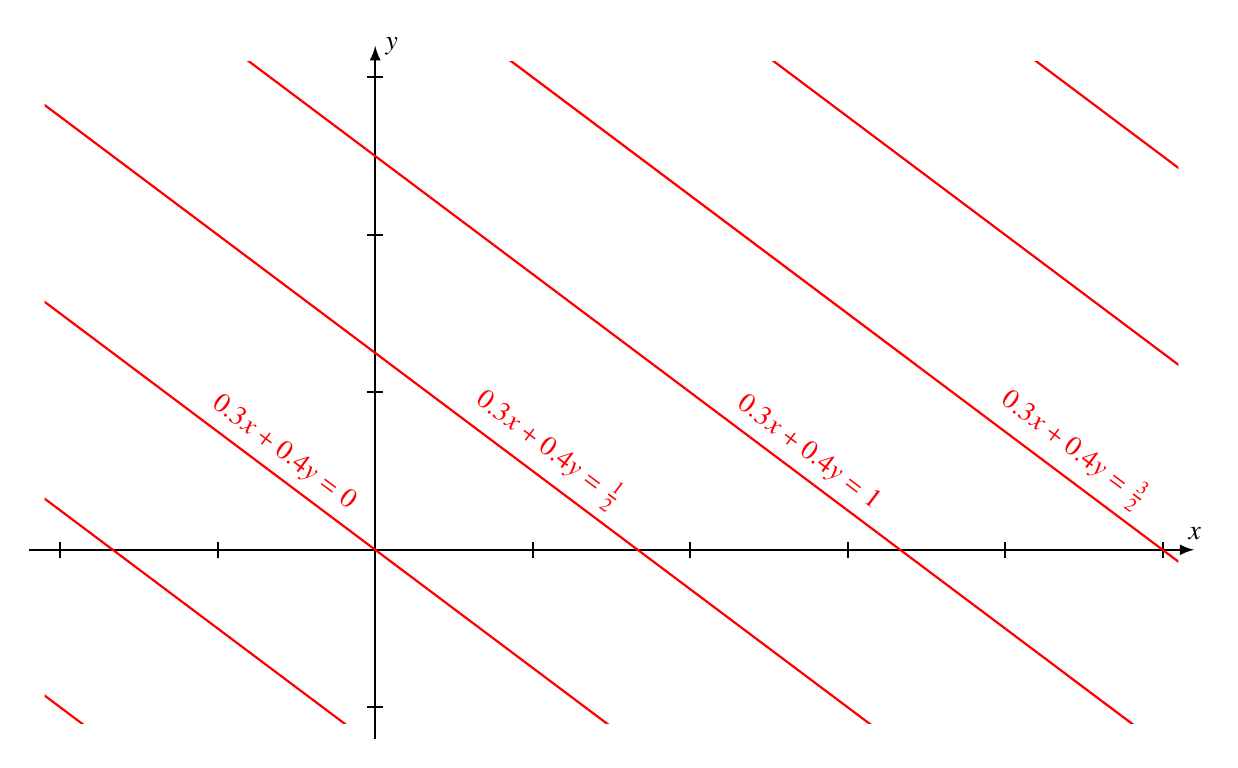
\begin{tikzpicture}[>=latex,thick]

\coordinate (O) at (0,0);

\draw[->] (-4.4,0)--(10.4,0) coordinate[label=$x$];
\draw[->] (0,-2.4)--(0,6.4) coordinate[label={right:$y$}];

\foreach \x in {-2,-1,...,5}{
	\draw ({2*\x},-0.1)--({2*\x},0.1);
}
\foreach \y in {-1,0,...,3}{
	\draw (-0.1,{2*\y})--(0.1,{2*\y});
}

\coordinate (N) at (0.3,0.4);
\coordinate (R) at (0.4,-0.3);
\coordinate (P) at (1.2,1.6);

\begin{scope}
\clip (-4.2,-2.2) rectangle (10.2,6.2);

\foreach \m in {-5,-4,...,5}{
	\draw[color=red] ($(O)-20*(R)+\m*(P)$)--($20*(R)+\m*(P)$);
}
\node[color=red] at (-1.333,1) [above,rotate={atan(-0.3/0.4)}] {$0.3x+0.4y=0$};
\node[color=red] at (2.,1) [above,rotate={atan(-0.3/0.4)}] {$0.3x+0.4y=\frac12$};
\node[color=red] at (5.333,1) [above,rotate={atan(-0.3/0.4)}] {$0.3x+0.4y=1$};
\node[color=red] at (8.666,1) [above,rotate={atan(-0.3/0.4)}] {$0.3x+0.4y=\frac32$};

\end{scope}

\end{tikzpicture}

\end{document}

